\begin{PROBLEM}
	\p
	% منبع اپدیا
	دو پشته با نام های 
	$A, B$
	داریم. یک عملیات به شرح زیر داریم:

	تا وقتی که حداقل دو عدد داخل 
	$A$
	موجود است، ازمیان دو عدد بالای 
	$A$
	عدد کوچک تر را انتخاب کرده و وارد 
	$B$
	می‌کنیم.
	در انتها نیز آخرین عدد 
	$A$
	را وارد
	$B$
	می‌کنیم.

	سپس تمام اعداد 
	$B$
	را از آن خارج کرده و به 
	$A$
	وارد می‌کنیم (توجه کنید چون 
	$A, B$
	پشته هستند با این کار اعداد با ترتیبی برعکس ترتیبشان در 
	$B$
	داخل
	$A$
	قرار خواهند گرفت)

	حال اگر عملیات گفته شده را 
	$1 \leq k \leq n$
	بار انجام دهیم به ازای چند جایگشت اولیه اعداد در 
	$A$
	این اعداد در انتهای کار مرتب خواهند بود؟

	برای فهمی بهتر عملیات به عکس زیر دقت کنید.
	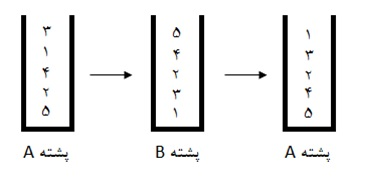
\includegraphics{18.jpg}
	
	\SOLUTION{
		\p

	}
\end{PROBLEM}